\documentclass[letterpaper,10pt,conference]{ieeeconf}

\IEEEoverridecommandlockouts
\overrideIEEEmargins

% ============================================================
% TETHER -- SUPPLEMENTARY MATERIAL
%
% Everything measured but cut from the 8-page submission.
% Every number here was produced by the same frozen checkpoint and the
% same evaluation code as the main paper; nothing was retrained or
% retuned to produce this document.
% ============================================================

\usepackage[T1]{fontenc}
\usepackage[utf8]{inputenc}
\usepackage{amsmath}
\usepackage{amssymb}
\usepackage{graphicx}
\usepackage{booktabs}
\usepackage{array}
\usepackage{multirow}
\usepackage{xcolor}
\usepackage{cite}
\usepackage{url}

\newcommand{\steer}{\textsc{TETHER}}
\newcommand{\raw}{\mathrm{raw}}
\newcommand{\mem}{\mathrm{mem}}
\newcommand{\fused}{\mathrm{fused}}
\newcommand{\TEPE}{\mathrm{TEPE}}

\title{\textbf{TETHER: Supplementary Material}}
\author{Anonymous Authors}

\begin{document}
\maketitle
\thispagestyle{empty}
\pagestyle{empty}

\begin{abstract}
This document reports measurements that did not fit the page limit. It
adds no claim to the main paper. Two of its sections
(Sec.~\ref{sup:tepe} and Sec.~\ref{sup:3d}) contain results that
\emph{qualify} the main claims rather than strengthen them, and they are
included for that reason.
\end{abstract}

% ============================================================
\section{Complete Matched-Baseline Closure}
\label{sec:closure}
% ============================================================

Table~\ref{sup:closure} lists all fifteen policies of the D2 closure.
The main paper reports a representative subset. Every row shares the
bounded state machine, the raw re-anchor schedule, the SEA-RAFT
alignment, the support definition and the fusion form; only the blending
weight differs, and all 225 reports (15 methods $\times$ 5 backbones
$\times$ 3 sequences) come from a single run under one frozen protocol.

\begin{table}[htb]
\centering
\small
\caption{Full SCARED-C D2 matched temporal-policy closure.
Raw EPE is $0.276202$. Positive reduction denotes improvement.}
\label{sup:closure}
\begin{tabular}{lrr}
\toprule
Method & EPE & Reduction \\
\midrule
\steer{} $H=6$ & \textbf{0.265893} & 3.73\% \\
\steer{} $H=4$ & 0.265998 & 3.69\% \\
\steer{} $H=8$ & 0.266473 & 3.52\% \\
\steer{} $H=2$ & 0.267858 & 3.02\% \\
\steer{} $H=1$ & 0.269331 & 2.49\% \\
\midrule
Fixed $w=0.5$ & 0.274562 & 0.59\% \\
EMA2          & 0.274562 & 0.59\% \\
Fixed $w=0.3$ & 0.274852 & 0.49\% \\
Fixed $w=0.2$ & 0.275229 & 0.35\% \\
EMA3          & 0.275386 & 0.30\% \\
Fixed $w=0.1$ & 0.275684 & 0.19\% \\
Warped raw previous    & 0.276298 & $-0.03\%$ \\
FB confidence weight   & 0.282182 & $-2.17\%$ \\
Warped recurrent $w=1$ & 0.286035 & $-3.56\%$ \\
Continuous recurrence  & 0.329140 & $-19.17\%$ \\
\midrule
Oracle raw/memory & 0.241023 & 12.74\% \\
\bottomrule
\end{tabular}
\end{table}

\paragraph{An identity worth stating.}
\texttt{EMA2} and \texttt{Fixed} $w=0.5$ are the same policy under two
names, and \texttt{EMA3} is $w=2/3$: under a recurrent state a fixed
convex weight \emph{is} an exponential moving average. The baseline
family is therefore five fixed weights
$w\in\{0.1,0.2,0.3,0.5,2/3\}$ over the shared bounded state, not two
independent families. We state this because two nominally different
baselines producing an identical number otherwise reads as a bug.

\subsection*{The Horizon Sweep, With Its Risk Side}

The main paper states that $H=4$ is a risk--gain operating point rather
than the EPE minimum, and points here for the sweep. The closure table
above gives the EPE column; this is the same sweep with the intervention
statistics that motivated the choice.

\begin{table}[!ht]
\centering
\footnotesize
\caption{Bounded horizon on D2. Lower EPE is better; higher $B^+/H^+$ and
lower NewBad1 are better.}
\label{sup:horizons}
\begin{tabular}{@{}lrrr@{}}
\toprule
$H$ & EPE & $B^+/H^+$ & NewBad1 (\%) \\
\midrule
1 & 0.269331 & 1.82 & 0.0518 \\
2 & 0.267858 & \textbf{1.85} & 0.0543 \\
4 & 0.265998 & \textbf{1.85} & 0.0627 \\
6 & \textbf{0.265893} & 1.74 & 0.0790 \\
8 & 0.266473 & 1.60 & 0.1282 \\
\bottomrule
\end{tabular}
\end{table}

The two columns disagree, and that disagreement is the whole reason the
operating point is not simply the EPE minimum. EPE bottoms out at $H=6$,
by $0.04$ points over $H=4$. Over the same step the beneficial-to-harmful
magnitude ratio falls from $1.85$ to $1.74$ and then to $1.60$, while
newly introduced Bad1 pixels rise from $0.0627\%$ to $0.0790\%$ to
$0.1282\%$ --- roughly doubling between $H=4$ and $H=8$. Letting the
corrected state live longer buys a sliver of mean accuracy and pays for
it in intervention risk.

$H=4$ was frozen on this trade before the held-out split was opened. We
report it as a choice rather than as an optimum, because on the metric
most papers would quote it is not one.

% ============================================================
\section{The Oracle Ceiling Is Not the One We Report Against}
% ============================================================

The oracle of the main paper selects, per pixel, the better of raw
disparity and aligned memory. It is therefore the ceiling of
$w\in\{0,1\}$, whereas \steer{} acts on $w\in[0,1]$, whose ceiling is
the continuous oracle
$w^{\star}=\mathrm{clip}\big((g-d^{\raw})/(\widetilde m-d^{\raw}),0,1\big)$.

\begin{table}[htb]
\centering
\small
\caption{Binary versus continuous oracle on D2, per backbone.}
\label{sup:oracle}
\begin{tabular}{lrrrr}
\toprule
Backbone & raw & \steer & $\{0,1\}$ & $[0,1]$ \\
\midrule
S$^2$M$^2$-S          & .2949 & .2858 & .2624 & .2599 \\
RAFT-Stereo           & .3022 & .2920 & .2675 & .2645 \\
Stereo Anywhere       & .3189 & .2974 & .2736 & .2708 \\
CREStereo             & .2943 & .2838 & .2597 & .2568 \\
Fast-FoundationStereo & .3037 & .2939 & .2702 & .2674 \\
\bottomrule
\end{tabular}
\end{table}

The correction is real but small. Only $6.4\%$ of D2 pixels have the
ground truth bracketed by the two candidates, so the two ceilings nearly
coincide and the recovered fraction falls from $33.8\%$ to $31.4\%$. We report it because the published figure is
measured against a ceiling the method cannot actually be limited by, not
because it changes the conclusion.

% ============================================================
\section{Motion-Compensated Multi-Horizon Fidelity}
\label{sup:tepe}
% ============================================================

$\TEPE_{\mathrm{corr}}$ and OPW require a correspondence field, supplied
here from the same SEA-RAFT flows used for warping. Table~\ref{sup:tepe}
gives the relative change after refinement, on the $142$-channel
configuration; the family is a diagnostic the paper does not build on, and the
shipped head is being measured on it separately.

\begin{table}[htb]
\centering
\small
\caption{$\TEPE_{\mathrm{corr}}$ (top) and OPW (bottom), relative change
after refinement. Negative is better.}
\label{sup:tepetab}
\begin{tabular}{llrrrr}
\toprule
Split & Backbone & $k{=}1$ & $k{=}2$ & $k{=}4$ & $k{=}8$ \\
\midrule
\multicolumn{6}{l}{\emph{$\TEPE_{\mathrm{corr}}$}}\\
D2 & S$^2$M$^2$-S          & +24.5\% & +40.1\% & +12.9\% & +19.7\% \\
D2 & RAFT-Stereo           & +24.8\% & +41.1\% & +16.6\% & +23.8\% \\
D2 & Stereo Anywhere       & +14.5\% & +31.1\% &  +8.5\% & +16.4\% \\
D2 & CREStereo             & +22.2\% & +39.7\% & +15.3\% & +24.3\% \\
D2 & Fast-FoundationStereo & +35.9\% & +52.3\% & +21.1\% & +27.8\% \\
D7 & S$^2$M$^2$-S          & -23.7\% & -21.0\% & -17.4\% & -12.7\% \\
D7 & RAFT-Stereo           & -12.2\% &  -6.1\% &  -5.6\% &  -5.7\% \\
D7 & Stereo Anywhere       & -10.3\% &  -4.8\% &  -5.3\% &  -5.7\% \\
D7 & CREStereo             & -13.6\% &  -6.8\% &  -6.7\% &  -6.4\% \\
D7 & Fast-FoundationStereo & -10.9\% &  -4.9\% &  -5.6\% &  -6.2\% \\
\midrule
\multicolumn{6}{l}{\emph{OPW}}\\
D2 & S$^2$M$^2$-S          &  -8.7\% &  -3.5\% &  -1.8\% &  -1.2\% \\
D2 & RAFT-Stereo           &  -8.5\% &  -3.4\% &  -1.7\% &  -1.1\% \\
D2 & Stereo Anywhere       & -12.9\% &  -5.8\% &  -3.0\% &  -1.8\% \\
D2 & CREStereo             &  -9.5\% &  -3.8\% &  -1.8\% &  -1.2\% \\
D2 & Fast-FoundationStereo &  -7.3\% &  -3.1\% &  -1.6\% &  -1.2\% \\
D7 & S$^2$M$^2$-S          & -29.8\% & -22.8\% & -13.5\% &  -7.6\% \\
D7 & RAFT-Stereo           & -18.5\% & -10.2\% &  -5.1\% &  -3.4\% \\
D7 & Stereo Anywhere       & -18.1\% &  -9.9\% &  -5.1\% &  -3.4\% \\
D7 & CREStereo             & -20.3\% & -11.1\% &  -5.9\% &  -3.8\% \\
D7 & Fast-FoundationStereo & -18.5\% & -10.0\% &  -5.2\% &  -3.6\% \\
\bottomrule
\end{tabular}
\end{table}

On held-out D7 both improve in all $20/20$ backbone--horizon cases. On
development D2 they disagree: OPW improves everywhere while
$\TEPE_{\mathrm{corr}}$ degrades everywhere.

This rules out a convenient explanation. One might attribute a rising
temporal-error metric to a grid metric penalising legitimate scene
motion, but $\TEPE_{\mathrm{corr}}$ \emph{is} motion compensated and
still degrades on D2. The two ask different questions: OPW asks whether
consecutive predictions agree with each other, $\TEPE_{\mathrm{corr}}$
whether the predicted temporal change matches the true one. On the split
used to select the operating point, the module therefore becomes more
self-consistent while tracking the true change less faithfully. We
report this against our own interest.

% ============================================================
\section{Forensics of the Support Violation}
% ============================================================

The main paper states that an unmasked output lets zero-padded
out-of-bounds memory become an invalid prediction. The supporting
measurement is below: every offending pixel has an aligned memory of
\emph{exactly} zero, and the offenders arrive in bursts no longer than
the state lifetime, so bounded recurrence contains the damage it cannot
prevent.

\begin{table}[htb]
\centering
\small
\caption{Invalid refined pixels under the unmasked output, and the state
age at which they occur.}
\label{sup:forensics}
\begin{tabular}{lrr}
\toprule
& Vid10\_Liver\_Med & Vid11\_Liver\_High \\
\midrule
Support pixels        & 38{,}828{,}160 & 38{,}439{,}360 \\
Invalid (unmasked)    & 300 & 265 \\
Invalid (support-confined) & \textbf{0} & \textbf{0} \\
Frames affected       & 10 & 3 \\
Aligned memory, min/max & $0.0$ / $0.0$ & $0.0$ / $0.0$ \\
Non-finite memory     & 0 & 0 \\
State age 1/2/3/4     & 10/103/135/52 & 0/182/72/11 \\
\bottomrule
\end{tabular}
\end{table}

Because an invalid prediction on valid support is penalised rather than
discarded, at $10^{4}$\,mm per pixel, a few hundred pixels out of
$38.8$~million decide the external-domain metric-depth verdict.

% ============================================================
\section{Per-Recording DRENDS Transfer}
% ============================================================

\begin{table}[htb]
\centering
\small
\caption{Zero-shot DRENDS, relative change after refinement, all metrics
and all five recordings. Negative is better.}
\label{sup:drends}
\begin{tabular}{llrrrr}
\toprule
Backbone & Recording & EPE & Bad3 & d.MAE & d.RMSE \\
\midrule
RAFT-Stereo & Vid10 & -6.0\% & -11.9\% & -4.0\% & -3.5\% \\
(seen)      & Vid11 & -3.9\% & -27.0\% & -2.8\% & -1.8\% \\
            & Vid12 & -9.1\% & -23.3\% & -7.3\% & -6.4\% \\
            & Vid13 & -4.5\% & -14.1\% & -3.3\% & -3.1\% \\
            & Vid14 & -4.7\% & -27.2\% & -3.7\% & -3.0\% \\
\midrule
CREStereo   & Vid10 & -5.3\% &  -9.4\% & -3.6\% & -3.7\% \\
(unseen)    & Vid11 & -4.2\% & -27.2\% & -3.0\% & -2.1\% \\
            & Vid12 & -7.2\% & -20.4\% & -5.6\% & -4.9\% \\
            & Vid13 & -5.5\% & -10.9\% & -3.8\% & -3.5\% \\
            & Vid14 & -5.9\% & -27.5\% & -4.5\% & -4.2\% \\
\midrule
Fast-Found. & Vid10 & -5.1\% &  -7.7\% & -3.2\% & -3.2\% \\
(unseen)    & Vid11 & -3.6\% & -24.3\% & -2.7\% & -1.9\% \\
            & Vid12 & -6.0\% & -11.1\% & -5.0\% & -4.0\% \\
            & Vid13 & -4.3\% & -10.3\% & -3.1\% & -2.9\% \\
            & Vid14 & -4.5\% & -25.6\% & -3.6\% & -2.9\% \\
\bottomrule
\end{tabular}
\end{table}

All 60 cells here improve, as do the other 40 the main paper aggregates
over. The per-recording pattern is set by the recording and not by the
estimator: on Vid10 the EPE change is $-6.0\%$, $-5.3\%$ and $-5.1\%$ for the
seen and the two unseen backbones. That alignment, rather than the pooled mean, is what
supports backbone independence.

% ============================================================
\section{Stage-Wise Runtime}
% ============================================================

NVIDIA H100 PCIe, PyTorch 2.5.1+cu121, $144\times180$ evidence grid, 200
timed iterations after 30 warmup iterations.

\begin{table}[htb]
\centering
\small
\caption{Per-stage temporal overhead, both configurations, measured in the
same session on an otherwise idle device.}
\label{sup:runtime}
\begin{tabular}{lrrr}
\toprule
Stage & \steer\ (ms) & p95 & $142$ ch (ms) \\
\midrule
SEA-RAFT forward & 13.088 & 13.238 & 13.173 \\
SEA-RAFT reverse & 13.089 & 13.186 & 13.174 \\
Alignment        & 1.049  & 1.067  & 1.058 \\
Evidence tensor  & 0.674  & 0.686  & 5.131 \\
Fusion head      & \textbf{1.002} & 1.012 & 1.014 \\
\midrule
Total overhead   & \textbf{28.903} & & 33.549 \\
Peak VRAM        & \textbf{95.2\,MB} & & 137.9\,MB \\
\bottomrule
\end{tabular}
\end{table}

Two observations. The $155$k-parameter head costs $1.00$\,ms, $3.5\%$ of the
overhead: ``compact head'' is true but not the operative cost, since $91\%$ is
the two frozen flow passes. And the reverse pass costs $13.09$\,ms while
feeding only the forward--backward confidence cue, whose direct use as a
fusion weight worsens EPE by $2.17\%$ (Table~\ref{sup:closure}); removing it
would cut overhead by $45\%$. Substituting a constant for the cue at inference
costs this head nothing measurable, which is reported in the main paper; a head
\emph{trained} without the reverse pass is still the experiment we have not
run. The evidence column is where the two configurations separate: $0.67$\,ms
against $5.13$, because \steer\ builds no learned features.

% ============================================================
\section{Three-Dimensional Surface Consistency}
\label{sup:3d}
% ============================================================

This section is superseded and kept for the record. It was written when we
believed SCARED-C carried no usable per-frame camera pose, so that global
reconstruction drift could not be measured; that belief was wrong, and the
world-frame measurement in the main paper --- which does accumulate geometry
in one frame using the corrected poses --- is the one that answers the
question this section could only approach. What follows instead back-projects
each frame's disparity to a metric cloud and compares it against the previous
frame's cloud pulled through the same SEA-RAFT correspondence: frame-to-frame
surface stability, not reconstruction drift. The numbers are the
$142$-channel configuration's; we have not re-run them on the shipped head,
because the measurement they belong to has been replaced rather than
updated.

\begin{table}[htb]
\centering
\small
\caption{Frame-to-frame 3D surface stability on D2, pooled means.
GT is the floor set by real scene and camera motion.}
\label{sup:3dtab}
\begin{tabular}{lrrr}
\toprule
Backbone & raw & refined & GT \\
\midrule
\multicolumn{4}{l}{\emph{point-to-point distance [mm]}}\\
S$^2$M$^2$-S          & 0.5016 & 0.4978 & 0.4758 \\
RAFT-Stereo           & 0.5085 & 0.5034 & 0.4758 \\
Stereo Anywhere       & 0.5060 & 0.4996 & 0.4758 \\
CREStereo             & 0.5065 & 0.5004 & 0.4758 \\
Fast-FoundationStereo & 0.4890 & 0.4902 & 0.4758 \\
\midrule
\multicolumn{4}{l}{\emph{surface-normal angle [deg]}}\\
S$^2$M$^2$-S          & 4.4878 & 4.3241 & 5.8586 \\
RAFT-Stereo           & 5.1443 & 4.7297 & 5.8586 \\
Stereo Anywhere       & 5.4499 & 4.8516 & 5.8586 \\
CREStereo             & 5.6006 & 4.9958 & 5.8586 \\
Fast-FoundationStereo & 3.7381 & 3.8742 & 5.8586 \\
\bottomrule
\end{tabular}
\end{table}

Excess over the GT floor falls on four backbones of five, for instance
$0.0326 \rightarrow 0.0276$\,mm on RAFT-Stereo, and rises slightly on
Fast-FoundationStereo. The effect is real but of the order of
$0.005$\,mm, which is why it never appeared in the paper even before the
world-frame measurement replaced it.

The normal metric carries a caveat that removes its floor entirely: GT
normals are \emph{noisier} than every prediction ($5.86^\circ$ against
$3.74$--$5.60^\circ$), because the pseudo-ground-truth is sparse and
central differences amplify it. Predictions smoother than the reference
cannot be scored against that reference, so the normal column should be
read as a relative comparison between raw and refined only.

Further assumptions a reader may wish to challenge: the principal point
is taken at the image centre with $f_y=f_x$, since the SCARED-C manifest
carries only $f_x$ and the baseline; flow correspondence stands in for
true scene-point correspondence, gated by forward--backward consistency
at library defaults; and both clouds live in their own camera frames, so
the measure mixes surface change with rigid camera motion, a component
the GT floor absorbs but does not isolate.

% ============================================================
\section{Larger Training Does Not Move the Operating Point}
% ============================================================

An augmented-training run keeps the architecture and enlarges the data. Both
arms here are the $142$-channel configuration, so this compares two training
regimes and not two heads; we have not repeated it on the shipped head.

\begin{table}[htb]
\centering
\small
\caption{Held-out D7, canonical versus augmented training.}
\label{sup:augmented}
\begin{tabular}{lrr}
\toprule
Metric & Canonical & Augmented \\
\midrule
Mean EPE & \textbf{.4693} & .4706 \\
HUR & \textbf{.3965} & .4457 \\
$H^{+}$ & \textbf{.0148} & .0235 \\
$B^{+}$ & .0376 & \textbf{.0450} \\
BUR & .4951 & \textbf{.5060} \\
Degraded-frame fraction & \textbf{.2642} & .3341 \\
Worst frame degradation & \textbf{.1063} & .3958 \\
\bottomrule
\end{tabular}
\end{table}

The augmented model performs more beneficial updates and substantially
more harmful ones. Scale shifts intervention aggressiveness without
improving held-out risk--gain balance.

% ============================================================
\section{External Stabiliser Context}
\label{sec:bida}
% ============================================================

BiDAStabilizer \cite{jing2024bida} is the closest published plug-in
stabiliser that can actually be run. The main paper reports the pooled
comparison; this section records how it was made fair and what it looks
like sequence by sequence.

Our first attempt was not comparable at all, for two independent reasons:
the published reproduction ran RAFT-Stereo \emph{robust} while we ran
RAFT-Stereo \emph{middlebury}, and it was scored under a different
support contract (raw EPE $0.3029$ against $0.2762$). Subtracting those
numbers would have been meaningless. Both differences are removed by
reading the stored NPZ boundary the reproduction already wrote --- the
exact RGB and the exact disparity BiDAStabilizer consumed --- running our
module on that same input, and scoring all three conditions against the
same ground truth on one prediction-independent support: GT coverage
$\cap$ raw validity, which neither method can influence. The one
remaining difference is the one that matters and is reported rather than
removed: BiDAStabilizer is bidirectional and consumes future frames.

\begin{table}[!htb]
\centering
\caption{Per-sequence common-support comparison, relative change against
raw (negative is better). Frames and support are identical within a row
group.}
\label{tab:bida_per_seq}
\setlength{\tabcolsep}{4pt}
\footnotesize
\begin{tabular}{@{}llrrr@{}}
\toprule
Sequence & Method & EPE & Bad1 & Bad3 \\
\midrule
keyframe\_2 & BiDAStabilizer & $\mathbf{-1.45}$ & $-4.01$ & $\mathbf{-5.31}$ \\
(1033 fr.)  & TETHER         & $-0.76$ & $\mathbf{-15.65}$ & $-4.00$ \\
\midrule
keyframe\_3 & BiDAStabilizer & $\mathbf{-2.32}$ & $-2.99$ & $\mathbf{-27.99}$ \\
(1102 fr.)  & TETHER         & $-0.38$ & $\mathbf{-4.81}$ & $-16.22$ \\
\midrule
keyframe\_4 & BiDAStabilizer & $+0.63$ & $-5.81$ & $-6.82$ \\
(2114 fr.)  & TETHER         & $\mathbf{-6.58}$ & $\mathbf{-17.76}$ & $\mathbf{-17.56}$ \\
\midrule
Pooled      & BiDAStabilizer & $-0.25$ & $-4.83$ & $-8.32$ \\
(18.0M px)  & TETHER         & $\mathbf{-4.60}$ & $\mathbf{-13.58}$ & $\mathbf{-16.81}$ \\
\bottomrule
\end{tabular}
\end{table}

The pooled row favours TETHER on every metric, but \emph{four} of the nine
per-sequence cells do not, and the bidirectional method takes both EPE cells
on the two shorter sequences. On \texttt{keyframe\_3} it improves EPE by
$2.32\%$ against our $0.38\%$, six times as much. The whole of our pooled EPE
margin comes from \texttt{keyframe\_4}, which is also the longest sequence and
carries half the pixels. We report this rather than pooling it away: with
three sequences that is well within what the split can produce, and a method
that sees the future should be expected to win somewhere. The claim the
comparison supports is the pooled one --- that a strictly causal module beats
a bidirectional one on the same input --- and not that it does so everywhere.

% ============================================================
\section{Acquisition Audit of the Comparison Set}
\label{sec:acq}
% ============================================================

The main paper states that no published method in our category can be run
head-to-head. That is a strong claim, so we record what was attempted, on
which date, and with what response. Everything below was checked on
16 August 2026 from the same host and the same session; the same
\texttt{curl} reached \texttt{huggingface.co} and \texttt{archive.org}
throughout, so a failure below is the resource's, not our network's.

\begin{table}[!htb]
\centering
\caption{What is actually obtainable. ``Category'' is causal $+$ black-box
$+$ attached to a frozen stereo network, which is our setting.}
\label{tab:acquisition}
\setlength{\tabcolsep}{3pt}
\footnotesize
\begin{tabular}{@{}llcc@{}}
\toprule
Method & Venue & Code & Weights \\
\midrule
StereoDiffusion \cite{xu2024stereodiffusion} & MICCAI'24 & none & none \\
Neural Disp.\ Refinement \cite{aleotti2021ndr} & 3DV'21 & yes & deleted \\
Lai et al. \cite{lai2018blind} & ECCV'18 & yes & host dead \\
TC-Stereo \cite{zeng2024tcstereo} & ECCV'24 & yes & yes \\
BiDAStabilizer \cite{jing2024bida} & ECCV'24 & yes & yes \\
\bottomrule
\end{tabular}
\end{table}

\paragraph{StereoDiffusion.} The only published method in our exact
category. Its repository has one commit, $7.43$\,KiB of git objects, and
contains a \texttt{.gitignore}, a \texttt{LICENSE} and a twelve-byte
\texttt{README.md}. \texttt{git ls-remote --heads} shows only
\texttt{main}. There is no implementation to run.

\paragraph{Neural Disparity Refinement.} Same input contract as ours
(RGB plus a black-box disparity), spatial only. The code clones and
imports. Both released Google Drive identifiers return HTTP 404 from
\texttt{drive.usercontent.google.com/download}, from
\texttt{docs.google.com/uc}, \emph{and} from the plain
\texttt{drive.google.com/file/d/.../view} landing page. A file that
exists but is access-restricted answers 403 or serves an interstitial;
404 on the landing page means the object is gone. Hugging Face model
search returns nothing for ``neural disparity refinement'' or
``disparity refinement''; the GitHub releases API for the official
repository returns an empty list; Zenodo returns zero records;
ModelScope has no such model.

\paragraph{Lai et al.} The natural task-agnostic baseline: model-agnostic
and causal at inference. Its
\texttt{pretrained\_models/download\_models.sh} points at
\texttt{vllab.ucmerced.edu}, which answers 200 for the directory listing
and 404 for every checkpoint. The Wayback CDX index holds the project
page, its stylesheets and the $34$\,MB supplementary PDF, and zero
captures of \texttt{ECCV18\_blind\_consistency.pth} or its optimiser
file --- web crawlers archive HTML and skip large binaries. No Hugging
Face mirror and no GitHub release exists.

\paragraph{TC-Stereo.} Obtainable and loadable: we found a configuration
that matches all three released checkpoints with zero missing and zero
unexpected keys ($16.7$\,M parameters). Its temporal branch warps the
previous disparity by a rigid $6$-DoF reprojection assembled from
per-frame camera pose, intrinsics and baseline.

We initially recorded that SCARED-C could not supply those poses. That
was wrong, and we correct it here: SCARED-C exists precisely because
SCARED's kinematics-propagated poses were too inaccurate, and it ships
COLMAP-re-estimated per-frame poses together with refined intrinsics
(\texttt{frame\_data.tar.gz}, \texttt{intrinsics\_colmap.yaml}). The
rigid-scene assumption is also reasonable on this data, which is ex-vivo:
the tissue is static and the endoscope moves. TC-Stereo's temporal path
is therefore runnable on SCARED-C, and the row below --- with the branch
disabled --- understates it a second time.

What remains true, and is the point worth making, is a difference in what
each method requires. TC-Stereo consumes per-frame $6$-DoF pose,
intrinsics and baseline; TETHER consumes RGB, disparity and validity. On
deformable data the rigid reprojection also stops being well-posed, which
is where our optical-flow alignment still applies. We report the
single-frame row as an integrated-architecture reference, and note the
temporal comparison as available future work rather than as impossible.

\paragraph{Deep Video Prior.} Excluded on definition rather than on
availability: it performs per-video test-time training over an entire
clip, so it is not causal under any configuration.

The practical consequence is that our comparison budget goes where a
comparison is actually possible: BiDAStabilizer on a common support
(Section~\ref{sec:bida}), TC-Stereo as the integrated reference, and the
matched-baseline closure of Section~\ref{sec:closure}, in which every
degenerate temporal policy shares our alignment, our support contract and
our evaluation code and differs only in the decision rule.

% ============================================================
\section{Seed Study in Full}
% ============================================================

Pre-registered before any seed result existed. The seed is the only field
that varies from the locked recipe; the training script is a sibling of
\texttt{train.py} that reuses its guards and overrides only that field.
The paired bootstrap resamples backbone--sequence cells, seeds are averaged
inside each resample, and four things were prohibited in advance:
selecting the best seed, re-tuning any threshold after seeing seed
results, changing the checkpoint-selection rule, and using D7 for any
decision other than the final reported numbers.

\begin{table}[!htb]
\centering
\caption{Relative Bad1 reduction (\%) per backbone over three seeds of the
\emph{$142$-channel} configuration, with the paired bootstrap interval and the
fraction of resamples in which refinement failed to help. This is the study
that found the development instability; the shipped head's own three seeds are
below.}
\label{tab:seeds_full}
\setlength{\tabcolsep}{3pt}
\scriptsize
\begin{tabular}{@{}llrrrrcr@{}}
\toprule
Split & Backbone & s0 & s1 & s2 & mean\,$\pm$\,std & CI$_{95}$ & $p$ \\
\midrule
D2 & CREStereo      &  8.26 &  6.62 &  3.57 & $6.15\pm2.38$ & $[0.69,12.74]$ & .000 \\
D2 & Fast-Found.    &  7.91 &  5.74 &  2.65 & $5.43\pm2.64$ & $[0.63,12.86]$ & .000 \\
D2 & RAFT-Stereo    &  6.95 &  5.40 &  3.00 & $5.12\pm1.99$ & $[-0.12,12.43]$ & .035 \\
D2 & S$^2$M$^2$-S   &  7.40 &  6.70 &  4.45 & $6.18\pm1.54$ & $[-0.31,12.32]$ & .038 \\
D2 & StereoAnywhere & 19.65 & 15.95 & 12.43 & $16.01\pm3.61$ & $[13.89,19.26]$ & .000 \\
\midrule
D7 & CREStereo      & 3.86 & 4.51 & 4.32 & $4.23\pm0.33$ & $[2.68,7.27]$ & .000 \\
D7 & Fast-Found.    & 3.97 & 4.08 & 3.76 & $3.93\pm0.16$ & $[1.60,8.58]$ & .000 \\
D7 & RAFT-Stereo    & 3.95 & 5.35 & 4.99 & $4.77\pm0.73$ & $[3.27,7.72]$ & .000 \\
D7 & S$^2$M$^2$-S   & 5.66 & 6.25 & 6.05 & $5.99\pm0.30$ & $[1.50,13.17]$ & .000 \\
D7 & StereoAnywhere & 6.40 & 7.07 & 6.73 & $6.73\pm0.33$ & $[5.66,12.12]$ & .000 \\
\midrule
\multicolumn{2}{@{}l}{Pooled, 35 sequences} & 5.79 & 6.00 & 5.28 & $5.69\pm0.37$ & $[4.11,8.02]$ & .000 \\
\bottomrule
\end{tabular}
\end{table}

Two features of this table are worth stating plainly rather than leaving
for a reader to find.

First, three D2 rows have intervals that touch or cross zero. That is a
property of the split, not of the method: D2 contributes three sequences,
and a three-sequence bootstrap is genuinely wide. We prefer reporting it
to quietly resampling pixels, which would have produced narrow intervals
with no statistical meaning. Held-out D7 contributes four sequences and
every one of its rows is strictly positive at $p=.000$ on both metrics.

Second, the seed ordering differs between splits in a way that is not
noise. Pooled per split, the D2 Bad1 reduction falls monotonically across
seeds --- $10.78$, $8.67$, $5.75$ --- while D7 gives $4.78$, $5.47$,
$5.19$, in which seed $0$ is the \emph{weakest}. Ten of ten per-backbone
comparisons follow the same direction. Our checkpoint-selection rule
picks best D2 fused EPE, so seed $0$ is by construction the run that
looked best on D2; the D2 margin therefore carries selection optimism and
the held-out margin does not.

\paragraph{The shipped head does not do this.} The same study on the
$38$-channel head, same recipe, same seeds, same rule:

\begin{table}[!htb]
\centering
\caption{Relative Bad1 reduction (\%) per backbone over three seeds of the
shipped head.}
\label{tab:seeds_a2}
\setlength{\tabcolsep}{3pt}
\scriptsize
\begin{tabular}{@{}llrrrr@{}}
\toprule
Split & Backbone & s0 & s1 & s2 & mean\,$\pm$\,std \\
\midrule
D2 & CREStereo      & 10.61 & 10.25 & 10.30 & $10.39\pm0.20$ \\
D2 & Fast-Found.    &  9.95 &  9.25 &  9.53 & $9.58\pm0.35$ \\
D2 & RAFT-Stereo    & 10.71 &  8.68 & 10.03 & $9.81\pm1.03$ \\
D2 & S$^2$M$^2$-S   &  9.13 &  9.57 &  9.68 & $9.46\pm0.29$ \\
D2 & StereoAnywhere & 20.51 & 20.71 & 21.69 & $20.97\pm0.63$ \\
\midrule
D7 & CREStereo      &  4.74 &  4.75 &  5.15 & $4.88\pm0.24$ \\
D7 & Fast-Found.    &  4.48 &  4.44 &  4.57 & $4.50\pm0.06$ \\
D7 & RAFT-Stereo    &  5.47 &  5.46 &  5.84 & $5.59\pm0.22$ \\
D7 & S$^2$M$^2$-S   &  6.40 &  6.42 &  6.94 & $6.58\pm0.31$ \\
D7 & StereoAnywhere &  7.31 &  7.53 &  7.86 & $7.56\pm0.28$ \\
\midrule
\multicolumn{2}{@{}l}{Pooled} & 12.84 & 12.38 & 12.98 & $12.73\pm0.32$ \\
\bottomrule
\end{tabular}
\end{table}

No monotone fall, no inversion, and the pooled D2 deviation is $0.32$ points
against the $2.53$ above. The instability was the evidence space, not the
selection rule --- which is unchanged between the two tables.

% ============================================================
\section{TC-Stereo as an Integrated Reference, and Why It Is Weak Evidence}
% ============================================================

TC-Stereo \cite{zeng2024tcstereo} is the one temporally-aware competitor
whose weights we obtained. Section~\ref{sec:acq} explains why its temporal
branch cannot run on SCARED-C: it warps the previous disparity by a rigid
$6$-DoF reprojection built from per-frame camera pose, which the dataset
does not provide and which deformable tissue would invalidate anyway. We
ran it with the temporal branch disabled --- its single-frame stereo path
--- over the same stored boundary as the BiDAStabilizer comparison, so the
frames and the ground truth are bit-identical across methods.

\begin{table}[!htb]
\centering
\caption{Same $4249$ frames, same ground truth, same support, $18.0$M
pixels. TC-Stereo is SceneFlow-pretrained and evaluated zero-shot with its
temporal branch disabled. Read the caveat below before using this row.}
\label{tab:tcstereo}
\setlength{\tabcolsep}{4pt}
\footnotesize
\begin{tabular}{@{}lrrrr@{}}
\toprule
Method & EPE & Bad1 (\%) & Bad3 (\%) & RMSE \\
\midrule
Raw RAFT-Stereo robust & 0.3029 & 2.087 & 0.186 & 0.4484 \\
BiDAStabilizer         & 0.3021 & 1.987 & 0.171 & 0.4403 \\
TETHER                 & \textbf{0.2889} & \textbf{1.804} & \textbf{0.155} & \textbf{0.4234} \\
\midrule
TC-Stereo (SceneFlow)  & 0.5242 & 9.051 & 1.680 & 1.4059 \\
\bottomrule
\end{tabular}
\end{table}

\paragraph{The caveat, which is large.} This row understates TC-Stereo and
we do not claim otherwise. The stored boundary is $144\times180$ with a
median ground-truth disparity of $8.04$\,px (range $5.57$--$15.53$),
whereas TC-Stereo was trained at full resolution on disparity ranges an
order of magnitude larger. Asking a from-scratch cost-volume matcher to
operate two octaves below its training regime is not a fair test of the
architecture. A refiner is far less exposed to this: BiDAStabilizer and
TETHER both consume the raw disparity and correct it, so the resolution
of the boundary constrains them much less than it constrains a matcher
built around a correlation pyramid.

We report the row anyway, with this caveat attached, because the
alternative --- running TC-Stereo at full resolution on frames the other
methods never saw --- would buy fairness to one method by destroying the
property that makes the whole table meaningful. The number is evidence
that swapping in a different integrated architecture zero-shot is not a
drop-in substitute for refining a strong in-domain frozen model. It is
\emph{not} evidence that TETHER outperforms TC-Stereo, and we make no such
claim.

\paragraph{One detail of the support.} We planned two supports, ground
truth alone and ground truth intersected with raw validity. On this
boundary they coincide exactly: \texttt{raw\_valid} is true everywhere, so
both conditions select the same $17{,}999{,}475$ pixels. The intersection
is reported as the definition because it is the one that would matter on a
boundary where the backbone declines pixels; here it is vacuous.

% ============================================================
\section{Analysis, in Full}
% ============================================================

The main paper compresses this section to a summary. Nothing here is
new evidence; it is the interpretation of results already reported,
kept intact because the page limit is on the submission and not on the
supplementary.

\paragraph{What Makes TETHER Work, and Why So Few Parameters Suffice}

The closure isolates four requirements. Geometric alignment is necessary
but not sufficient: the aligned memory carries a $12.74\%$ oracle
ceiling, yet using it indiscriminately fails, since warped raw memory
yields no meaningful gain and both direct FB-confidence weighting and
full recurrent replacement worsen EPE. Under identical evidence and
support the learned policy obtains more than six times the gain of the
best fixed blend, and the recurrent state must stay bounded because
continuous propagation accumulates error and collapses. The mechanism is
motion alignment plus learned graded intervention plus bounded recurrent
state, not generic smoothing.

This also explains the parameter count. The head never solves stereo
matching: it receives two already meaningful candidates, $d_t^{\raw}$ and
$\widetilde m_t$, plus evidence describing their disagreement, motion
reliability and validity, so its problem is closer to judging whether
temporal evidence is useful than to predicting disparity from RGB. Convex
fusion further restricts the action space to a position between the two
candidate geometries. We previously offered that constraint as a plausible
reason why one small head transfers to unseen architectures. The
pre-registration required that claim to be withdrawn rather than softened if
the relaxed-convexity ablation matched or beat the canonical model on the
held-out endpoint. It did, by the largest margin in the table, so the claim is
withdrawn: we do not know why the head transfers.

\paragraph{The Oracle Gap Is the Next Problem}

TETHER captures $33.8\%$ of the raw-versus-memory oracle gain and
$31.4\%$ of the continuous oracle its convex action space could reach;
only $6.4\%$ of D2 pixels have the ground truth bracketed by the two
candidates, so the ceilings nearly coincide. Useful evidence already
exists; the open problem is discriminating helpful from harmful
intervention.

\paragraph{The Fusion Weight Is Not an Uncertainty}

Recovering the effective weight exactly from the convex form,
$w_t=(d_t^{\fused}-d_t^{\raw})/(\widetilde m_t-d_t^{\raw})$, and scoring
it as a predictor of harmful intervention gives AUROC $0.393$--$0.408$ on
D2 --- below chance on the split it was selected on --- and
$0.488$--$0.507$ on held-out D7, i.e.\ chance; the raw--memory
disagreement and the update magnitude behave the same way. The
reliability curve inverts between splits --- for RAFT-Stereo, across the
populated weight bins, the harm rate \emph{falls} with $w_t$ on D2
($0.396\rightarrow0.287$) and \emph{rises} on D7
($0.250\rightarrow0.362$) --- so $w_t$ is not a weak risk score but a
sign-unstable one, and a threshold tuned on development would select the
wrong pixels held out. It is an intervention magnitude, not an uncertainty,
and closing the oracle gap needs evidence the head does not receive.

\paragraph{Reconciling this with the intervention table}

Taken alone, the previous paragraph appears to contradict the
intervention-quality table of the main paper: if $w_t$ carries no information
about harm on D7, how does the same policy reach $B^+/H^+$ between
$2.18$ and $3.64$ there? The two statements are about different things,
and the aggregate gain factorises exactly into them. Writing
$\delta e = e^{\fused}-e^{\raw}$ per intervened pixel,
%
\begin{equation}
\frac{B^+}{H^+}
=\underbrace{\frac{\#\{\delta e<0\}}{\#\{\delta e>0\}}}_{\text{count}}
\times
\underbrace{\frac{\mathbb{E}[|\delta e| \mid \delta e<0]}
                 {\mathbb{E}[|\delta e| \mid \delta e>0]}}_{\text{magnitude}} .
\label{eq:factorisation}
\end{equation}
%
Pooled over the five backbones this evaluates to $2.861=1.294\times2.212$
on held-out D7 and $2.028=1.114\times1.820$ on D2. On D7, $56.4\%$ of
interventions improve the pixel and the improvements are $2.2\times$ larger
than the regressions.

Neither factor requires $w_t$ to rank anything. The policy shifts the
\emph{distribution} of $\delta e$ favourably, which is what
that table measures; the AUROC asks the
strictly harder question of whether the scalar the head emits identifies
\emph{which} pixels fall in the harmful $43.6\%$, and on held-out data it
does not. A policy can be reliably good on average and completely
uninformative per pixel: those are independent properties, and TETHER has
the first without the second.

This sharpens rather than weakens the oracle-gap claim. The remaining
$67\%$ of the oracle is not reachable by thresholding anything the head
already computes, because the quantity it computes is a magnitude and the
gap is a ranking problem.


\paragraph{Evaluation Matters}

The framework exposes behaviour a mean would hide: on DRENDS mean and
percentile geometry improve while RMSE worsens; longer horizons slightly
improve mean D2 EPE while degrading $B^+/H^+$, NewBad1 and the frame
tails. Temporal refinement is better read as an \emph{intervention} than
as a final estimator.

One reported quantity failed an audit and is withdrawn: FrameDegradation's
CatastrophicFraction is definitionally identical to PositiveFraction at
the default threshold, so we report only the degraded-frame fraction
$\Pr(D_t>0)$. The supplementary gives the derivation.

% ============================================================
\section{Intervention Quality per Backbone}
% ============================================================

The main paper quotes the ranges; this is the table behind them. $B^+/H^+$ is the beneficial-to-harmful error-magnitude ratio and ``Rec./New'' the ratio of recovered to newly introduced Bad1 pixels, both on the prediction-independent protocol support.

\begin{table}[!htb]
\centering
\scriptsize
\caption{
TETHER intervention quality, seed $0$.
All ratios exceed one; higher is better.
``Rec./New'' is RecoveredBad1/NewBad1.
}
\label{tab:intervention_quality}
\begin{tabular}{lrrrr}
\toprule
& \multicolumn{2}{c}{D2} & \multicolumn{2}{c}{D7} \\
\cmidrule(lr){2-3}\cmidrule(lr){4-5}
Backbone & $B^+/H^+$ & Rec./New & $B^+/H^+$ & Rec./New \\
\midrule
S$^2$M$^2$-S          & 1.39 & 3.8$\times$  & 2.16 & 7.5$\times$ \\
RAFT-Stereo           & 1.58 & 4.9$\times$  & 2.92 & 4.7$\times$ \\
Stereo Anywhere       & 3.07 & 9.9$\times$  & 3.25 & 11.1$\times$ \\
CREStereo             & 1.70 & 5.0$\times$  & 2.57 & 4.7$\times$ \\
Fast-FoundationStereo & 1.57 & 5.3$\times$  & 2.26 & 7.8$\times$ \\
\bottomrule
\end{tabular}
\end{table}

% ============================================================
\section{Ablations in Full}
\label{sec:ablations_full}
% ============================================================

The main paper reports held-out EPE and Bad1 for the four pre-registered
ablations. This is the same evaluation on both splits and four metrics.

\begin{table}[!ht]
\centering
\caption{Relative reduction (\%) against the same raw predictions. The raw
baseline is identical to six decimals across all six runs, so the rows are
directly comparable. Canonical, A2 and A3 are means of three seeds; A1 and A4
are single runs. ``Canonical'' is the $142$-channel configuration the
deviations were registered against; A2 is the head the paper ships.}
\label{tab:ablations_full}
\setlength{\tabcolsep}{3pt}
\scriptsize
\begin{tabular}{@{}lrrrrrrrr@{}}
\toprule
& \multicolumn{4}{c}{D2 development} & \multicolumn{4}{c}{D7 held out} \\
\cmidrule(lr){2-5}\cmidrule(lr){6-9}
& EPE & Bad1 & Bad3 & RMSE & EPE & Bad1 & Bad3 & RMSE \\
\midrule
Canonical & 3.55 & 8.40 & 16.71 & 12.97 & 5.06 & 5.15 & 4.29 & 5.60 \\
A1 & 4.18 & 8.81 & 15.76 & 13.11 & 4.93 & 4.88 & 4.12 & 5.46 \\
A2 & 4.13 & 12.73 & 19.64 & 13.87 & 5.61 & 5.84 & 5.18 & 6.02 \\
A3 & 3.85 & 8.10 & 18.34 & 13.10 & 5.24 & 5.68 & 5.53 & 5.89 \\
A4 & 5.53 & 12.44 & 19.26 & 13.58 & 0.05 & 6.02 & 5.32 & 6.32 \\
\bottomrule
\end{tabular}
\end{table}

Three things are visible here that the main table has no room for.

First, A4's failure is specific rather than general. It is the best
variant in the table on Bad1, Bad3 and RMSE on \emph{both} splits, and
its held-out EPE gain is $0.05\%$. A quadratic metric improving while a
linear one collapses rules out occasional large errors --- outliers hurt
RMSE first --- and leaves broad degradation of pixels that were already
close, which the mean registers and thresholds and squared errors do not.

Second, A1 and A2 differ in a way that makes them one experiment rather
than two. A1 removes the $64$ raw appearance channels but keeps the
appearance self- and cross-correlations computed from those same
features; it is indistinguishable from canonical. A2 removes the
correlations as well, and is better on all four held-out metrics. The
more appearance-derived evidence leaves the interface, the better the
head generalises --- which is what one would expect of evidence that ties
the decision to the training domain.

Third, D2 and D7 disagree about A1. On D2 it is close to canonical on
Bad1 ($8.81$ against $8.40$) but better on EPE ($4.18$ against $3.55$); on
D7 it is $0.27$ points below on the registered endpoint, inside the
$0.37$-point threshold and so unreadable rather than worse. This is the same
development-versus-held-out inversion the seed study found, and it is the
reason the pre-registration named a held-out endpoint before any variant
was trained.

\paragraph{What happened next.} A2 was the strongest variant and was not
promoted on the strength of a held-out win, because choosing on the held-out
split is what makes a held-out split stop being one. It was given the same
three-seed treatment the canonical model
has, and the comparison that could promote it was fixed on D2, the
development split, before those seeds were trained. It cleared that bar by
$4.33$ points with a comparable spread, so it was promoted, and it is the
head the main paper proposes. A3 was then given the same three-seed treatment
for the opposite reason --- it beat its base by more than the declared
threshold on the registered endpoint --- and it still does
($5.68\pm0.16$ against $5.15\pm0.34$). We decline it on the $16\times$
context-branch compute rather than on accuracy, and say so in the main
paper rather than presenting the rejection as an evidential one.

% ============================================================
\section{A Metric Field We Do Not Report}
% ============================================================

FrameDegradation's CatastrophicFraction was numerically identical to
PositiveFraction on every inspected row. The cause is definitional:
the two are $\Pr(D_t>\tau_{\mathrm{cat}})$ and $\Pr(D_t>0)$, and the
catastrophic threshold defaults to $\tau_{\mathrm{cat}}=0$, which the
evaluators never override. At that setting they coincide by
construction. We therefore report only the degraded-frame fraction,
defined explicitly as $\Pr(D_t>0)$.

\begin{thebibliography}{9}
\bibitem{jing2024bida}
J.~Jing, Y.~Mao, A.~Qiu, and K.~Mikolajczyk,
``Match Stereo Videos via Bidirectional Alignment,''
in \emph{Proc. European Conf. Computer Vision (ECCV)}, 2024.
\bibitem{xu2024stereodiffusion}
H.~Xu, C.~Xu, and S.~Giannarou,
``StereoDiffusion: Temporally consistent stereo depth estimation with diffusion models,''
in \emph{Proc. MICCAI}, 2024.
\bibitem{aleotti2021ndr}
F.~Aleotti \emph{et al.},
``Neural disparity refinement for arbitrary resolution stereo,''
in \emph{Proc. Int. Conf. 3D Vision (3DV)}, 2021.
\bibitem{lai2018blind}
W.-S.~Lai \emph{et al.},
``Learning blind video temporal consistency,''
in \emph{Proc. European Conf. Computer Vision (ECCV)}, 2018.
\bibitem{zeng2024tcstereo}
Z.~Zeng \emph{et al.},
``Temporally consistent stereo matching,''
in \emph{Proc. European Conf. Computer Vision (ECCV)}, 2024.
\end{thebibliography}


\section{Material Moved from the Main Paper}

The main paper is eight pages. Four objects that were in it are now here in
full, and nothing measured was deleted to make room.

\paragraph{Table: out-of-domain head-to-head with BiDAStabilizer.}
Five DRENDS recordings, $117.4$M pixels of common support, neither method in
domain.

\begin{center}
\begin{tabular}{lccccccc}
\toprule
Method & Causal & EPE & Bad1 (\%) & Bad3 (\%) & RMSE & $\mathrm{DTCE}_1$ & $\mathrm{DTCE}_4$ \\
\midrule
Raw            & ---          & $1.199$ & $44.92$ & $4.54$ & $1.876$ & $0.242$ & $0.340$ \\
BiDAStabilizer & no           & $1.175$ & $44.81$ & $4.32$ & $1.776$ & $\mathbf{0.085}$ & $\mathbf{0.214}$ \\
TETHER         & \textbf{yes} & $\mathbf{1.131}$ & $\mathbf{43.39}$ & $\mathbf{3.94}$ & $\mathbf{1.710}$ & $0.139$ & $0.294$ \\
\bottomrule
\end{tabular}
\end{center}

The two best columns belong to different rows. The bidirectional baseline is
the more temporally stable method and the less accurate one, at every lag and
in each of the five recordings.

\paragraph{Table: per-backbone DRENDS transfer.}
Relative change in \%, negative is better; each entry is the mean over the
five recordings.

\begin{center}
\begin{tabular}{llrrrr}
\toprule
Backbone & Status & EPE & Bad3 & Depth MAE & Depth RMSE \\
\midrule
S$^2$M$^2$-S          & seen   & $-4.86$ & $-18.44$ & $-3.65$ & $-3.06$ \\
RAFT-Stereo           & seen   & $-5.63$ & $-20.71$ & $-4.22$ & $-3.58$ \\
Stereo Anywhere       & seen   & $-6.21$ & $-23.54$ & $-4.60$ & $-4.09$ \\
CREStereo             & unseen & $-5.62$ & $-19.07$ & $-4.12$ & $-3.67$ \\
Fast-FoundationStereo & unseen & $-4.70$ & $-15.80$ & $-3.50$ & $-2.97$ \\
\midrule
All $25$ cells        &        & $-5.40$ & $-19.51$ & $-4.02$ & $-3.47$ \\
\bottomrule
\end{tabular}
\end{center}

\paragraph{Figure: per-frame Bad1 scatter.}
Raw against refined for every scored frame of each split --- five backbones,
all sequences, no selection. On held-out D7, $56\%$ of $15{,}535$ frames
improve against $14\%$ worsened; on development D2, $45\%$ against $18\%$.
The worsened band hugs the diagonal while the improved mass extends far from
it, which is the count-versus-magnitude asymmetry behind $B^+/H^+$.

\begin{center}
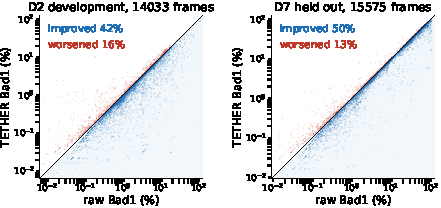
\includegraphics[width=0.62\columnwidth]{frame_scatter.pdf}
\end{center}

\paragraph{TC-Stereo, evidence-space construction, head widths, stage timing.}
These already have sections of their own above.

\end{document}
